\documentclass[english, 12pt]{beamer}
% Add handout to documentclass options if wanted

\usepackage[utf8]{inputenc}
\usepackage[T1]{fontenc}
\usepackage{babel,textcomp}


\usepackage{graphicx}
\usepackage{amsmath}
\usepackage{amssymb}
\usepackage{amsbsy}
\usepackage{amsfonts}
\usepackage{color}
\usepackage{xcolor}
\usepackage{epstopdf}
\usepackage{fancyvrb}
\usepackage{parskip}
\usepackage{url}
\usepackage{listings}

\DeclareMathAlphabet{\mathbfit}{OML}{cmm}{b}{it}

\definecolor{javared}{rgb}{0.6,0,0} % for strings
\definecolor{javagreen}{rgb}{0.25,0.5,0.35} % comments
\definecolor{javapurple}{rgb}{0.5,0,0.35} % keywords
\definecolor{javadocblue}{rgb}{0.25,0.35,0.75} % javadoc

\lstset{language=python,
basicstyle=\ttfamily\scriptsize,
keywordstyle=\color{javapurple},%\bfseries,
stringstyle=\color{javared},
commentstyle=\color{javagreen},
morecomment=[s][\color{javadocblue}]{/**}{*/},
% numbers=left,
% numberstyle=\tiny\color{black},
stepnumber=2,
numbersep=10pt,
tabsize=4,
showspaces=false,
captionpos=b,
showstringspaces=false,
frame= single,
breaklines=true}


\setlength{\arrayrulewidth}{1.6pt}
\renewcommand{\arraystretch}{1.2}
\newlength{\Tcalc}


\setbeamertemplate{frametitle}
{\begin{centering}\smallskip
\insertframetitle\par
\smallskip\end{centering}}
\setbeamertemplate{itemize item}{$\bullet$}
\setbeamertemplate{navigation symbols}{}
\setbeamertemplate{footline}[text line]{%
\hfill\strut{%
\scriptsize\sf\color{black!60}%
\quad\insertframenumber
   }%
    \hfill
}

% Define some colors:
\definecolor{DarkFern}{HTML}{407428}
\definecolor{DarkCharcoal}{HTML}{4D4944}
\colorlet{Fern}{DarkFern!85!white}
\colorlet{Charcoal}{DarkCharcoal!85!white}
\colorlet{LightCharcoal}{Charcoal!50!white}
\colorlet{AlertColor}{orange!70!black}
\colorlet{DarkRed}{red!70!black}
\colorlet{LightBlue}{blue!70!white}
\colorlet{DarkBlue}{blue!70!black}
\colorlet{DarkGreen}{green!70!black}

% Use the colors:
\setbeamercolor{title}{fg=Fern}
\setbeamercolor{frametitle}{fg=Fern}
\setbeamercolor{normal text}{fg=Charcoal}
\setbeamercolor{block title}{fg=black,bg=Fern!25!white}
\setbeamercolor{block body}{fg=black,bg=Fern!25!white}
\setbeamercolor{alerted text}{fg=AlertColor}
\setbeamercolor{itemize item}{fg=Charcoal}

\newcommand{\frn}[1]{\textcolor{Fern}{#1}}
\newcommand{\alrt}{\color{AlertColor}}
\newcommand{\bt}[1]{\textbf{#1}}
\newcommand{\kommando}[1]{\textcolor{AlertColor}{\texttt{\textbackslash #1}}}
\newcommand{\ds}{\displaystyle}

\renewcommand{\d}{\textrm{d}}

\title{Programmeringsprosjekt Sandvika \\ {\small En introduksjon til numeriske beregninger}}
\author{Jonas van den Brink \\ \texttt{j.v.brink@fys.uio.no}}
\institute{\alrt Simula Research Laboratory \\ Oslo, Norway}

\setbeamertemplate{frametitle}{\vspace{0.5cm} \insertframetitle} 

\begin{document}
\pagestyle{empty}

\begin{frame}[fragile]
\frametitle{Algoritme for Eulers metode}
for $i=0,1,2,3,\ldots, N-1$:
\begin{enumerate}
	\item Bruk de forrige resultatene $x_i$ og $v_i$ for å regne ut akselerasjonen: $\alrt a_i = F(x_i, v_i, t_i)/m$.
	\item Regn ut den nye farten: $\alrt v_{i+1} = v_i + a_i\Delta t$.
	\item Regn ut den nye posisjonen: $\alrt x_{i+1} = x_i + v_i\Delta t + \frac{1}{2}a_i\Delta t^2$.
\end{enumerate}
\visible<2-> {
$$\Downarrow$$

\lstinputlisting{lsteuler.py}
$$\alrt t_i \Rightarrow \texttt{t[i]} \qquad  v_i \Rightarrow \texttt{v[i]} \qquad  r_i  \Rightarrow \texttt{r[i]}$$
}
\end{frame}

\begin{frame}
\lstinputlisting{shell.py}
\end{frame}

\begin{frame}
\lstinputlisting{shell2.py}
\end{frame}

\begin{frame}
\frametitle{Luftmotstand}

$$\alrt F_d = -\frac{1}{2}\rho C_D A  |v|v.$$

\end{frame}

\begin{frame}
\begin{center}
\begin{tabular}{c|c}
\quad Fritt Fall \quad \quad\\ \hline
$m$ & 90 kg \\ \hline
$g$ & 9.81 m/s$^2$ \\ \hline
$\rho$ & 1 kg/m$^3$\\ \hline
$C$ & 1.4 \\ \hline
$A$ & 0.7 m$^2$\\ 
\end{tabular}

\begin{tabular}{c|c}
Under fallskjerm \\ \hline
$C_{\rm p}$ & \quad \ 1.8 \qquad \qquad \\ \hline
$A_{\rm p}$ & 44 m$^2$
\end{tabular}
\end{center}
\end{frame}

\begin{frame}
\frametitle{Oppgave 1}

Skriv koden for å simulere en fallskjermhopper i fritt fall, ikke tenk på fallskjermen enda. Anta at hoppet starter ved 4000 meters høyden, og anta at hopperen starter med null hastighet mot bakken. Simuler fallskjermhopperen i 1 minutt.

\begin{itemize}
	\item[(a)] Plot absoluttverdien av farten, $\alrt |v|$. \\\textbf{Hint: Du kan bruke \texttt{\alrt abs(v)} for absoluttverdien.} 
	\item[(b)] Hva er terminalhastigheten (maksfarten) til hopperne? Hvor lang tid tar det ca før hopperen når den farten?
	\item[(c)] Plot fallskjermhopperens høyde over bakken mot tid. 
	\item[(d)] Hvor høyt over bakken er fallskjermhopperen etter 1 minutt i fritt fall? Hvor lang tid vil det ta før hopperen treffer bakken med denne farten?
\end{itemize}
\end{frame}

\begin{frame}[fragile]
\frametitle{La oss snakke om $g$-krefter}	

\visible<2->{
Tross navnet, er $g$-krefter et mål på \emph{\alrt akselerasjon}, ikke krefter. Det er definert som akselerasjonen fra summen av alle kontaktkrefter (altså \emph{ikke} gravitasjon) målt i antall $\alrt g$.}

\vspace{0.6cm}

\visible<3->{
Til vanlig føler vi $\alrt 1g$, fra kontaktkraften fra gulvet eller stolen. Hvis du føler $\alrt 0g$ er du i fritt fall, det føler du for eksempel i stupet på en berg-og-dalbane.
}

\vspace{0.6cm}

\visible<4->{
Vi kan lett regne ut $g$-kreftene iløpet av bevegelsen
\lstinputlisting{gforces.py}
}
\end{frame}



\begin{frame}
\frametitle{Oppgave 2}

La oss ta hensyn til fallskjermen. Vi simulerer de første 60 sekundene likt som istad. Når tiden når 60 sekunder, `løser' vi ut fallskjermen ved å endre parametrene $C_D$ og $A$.

\begin{itemize}
    \item[(a)] I Euler-løkka, legg inn en \texttt{\alrt if}-test som endrer $C_D$ og $A$ når tiden når 60 sekunder. Simuler hopperen i 2 minutter.\\  \textbf{Hint: \texttt{\alrt if 60.\ < t[i] < 60.\ + dt:}}
	\item[(b)] Plot hastigheten og høyden over bakken.
	\item[(c)] Hvor høyt over bakken er fallskjermhopperen etter 2 minutter? Ca hvor lenge til er det hun treffer bakken?
	\item[(d)] Hva er terminalhastigheten med fallskjermen utløst?
	\item[(e)] Plot $g$-kreftene som hopperen føler iløpet av hoppet. Diskuter med sidemannen og forklar endringene i $g$-kreftene. Er det realistisk? Hvorfor/Hvorfor ikke?
\end{itemize}
\end{frame}

\begin{frame}
\frametitle{Oppgave 3}

I forrige oppgave ble $g$-kreftene \emph{altfor} store. De ville garantert drept enhver hopper. Problemet er at vi `løste' ut fallskjermen altfor fort. Istedet for å endre parameteren rett fra en verdi til en annen, la oss endre dem over et par sekunder:
\lstinputlisting{release.py}

\begin{itemize}
	\item[(a)] Endre koden som foreslått. Simuler helt til fallskjermhopperen når bakken.
	\item[(b)] Hva er nå maks $g$-krefter hopperen opplever?
\end{itemize}
\end{frame}

\begin{frame}
\frametitle{Fjærkraft}
\begin{center}
	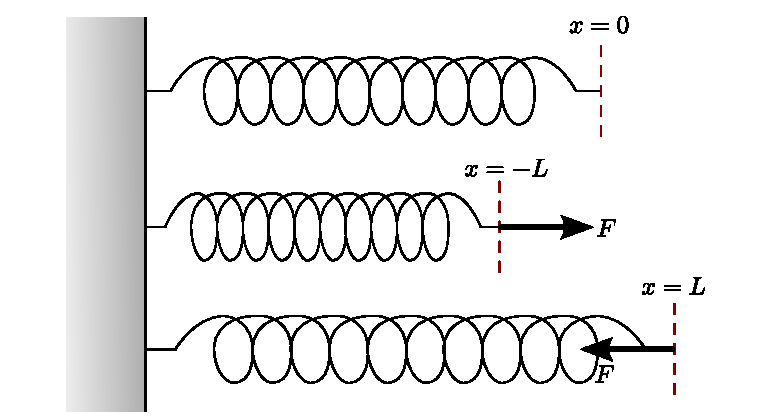
\includegraphics[width=\textwidth]{spring.pdf}
\end{center}

$$\alrt F_k = -kx \qquad \mbox{(Hookes lov)}$$ 
\end{frame}

\begin{frame}
\frametitle{Strikkkraft}
Strikkhopp er med en strikk, og ikke en fjær. En strikk ligner mye på en fjær, men virker bare `en vei'.

$$\alrt F_k = \begin{cases}
-kx & \mbox{if } x > 0 \\
0 & \mbox {if } x < 0.
\end{cases}
$$
\end{frame}

\begin{frame}
\frametitle{Strikkhopp}
\begin{center}
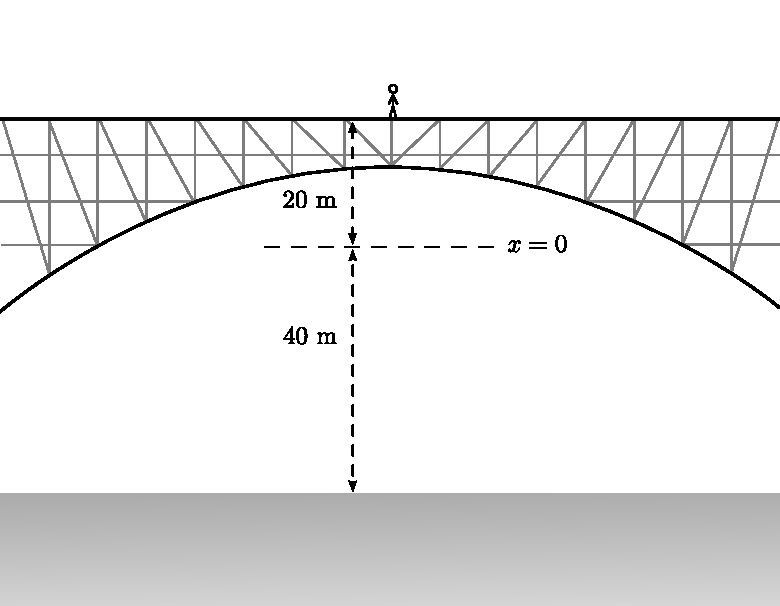
\includegraphics[width=\textwidth]{Bungee_bridge}
\end{center}
\end{frame}

\begin{frame}
\frametitle{Oppgave 4}

Kopier fallskjermhopp programmet ditt, og endre det så det gjelder for strikkhopp istedet. Gjett på en fjærstivhet, reduser massen til det du selv veier. Start hoppet fra $20$ meter over likevektspunktet, anta at elven er 60 meter under brua (altså starter vannet på $-40$ meter). 

\begin{itemize}
	\item[(a)] Prøv deg frem til du finner en fjærstivhet som gjør at du akkurat `toucher' vannet.
	\item[(b)] Hvor mange sekunder tar det fra du hopper fra brua til du treffer vannet?
	\item[(c)] Simuler bevegelsen i flere minutter, ser bevegelsen realistisk ut? Hva kan gjøre at det ikke er helt realistisk? Diskuter med sidemannen.
	\item[(d)] Plot $g$-kreftene. Sammenlign med fallskjermhopp
\end{itemize}

\end{frame}


\end{document}